\subsection{}
First let us extend the alphabet $\Sigma$ to $\Sigma' = \Sigma \cup \{\epsilon\}$ where $\epsilon$ is the empty sting. Now, for each state $s\in S$, $e_s(\epsilon) = 1 - \sum_{a\in \Sigma} e_s(a)$ hence $\sum_{a\in \Sigma'} e_s(a) = 1$. Using epsilon we can now consider the problem as finding the most likely sequence of states to generate our sequence, $O$, of $n$ symbols with any number of $\epsilon$ in $O$ at any position.

The Viterbi Algorithm $\delta$ can be described mathematically as:
\begin{align*}
\textbf{Base Case: } &\delta_1(i) = \pi_i e_i(O_1)\\
\textbf{Inductive Case: } &\delta_t(j) = \max_{1\leq i \leq N}[\delta_{t-1}(i)m_{ij}]\cdot e_j(O_t)
\end{align*}

Our new algorithm will extend the Viterbi algorithm. As a high level explanation, our new algorithm will no longer assume in the inductive step that we directly transition from state $i$ to $j$ with probability $m_{ij}$. 
Instead it will allow any path from $i$ to $j$, where if we travel through an intermediate state it will emit $\epsilon$.
Given we are finding the most likely sequence of states we need only consider the most likely path from $i$ to $j$. 
To describe this path we will define $\psi(i,j)$ as the path of maximum likelihood from $i$ to $j$ where transitions $x$ to $y$ must emit $\epsilon$ unless $x=i$ (as we know $i$ has already emitted symbol $O_t$).

You can calculate $\psi$ using Dijksta's algorithm. To do this we will use Dijkstra's to find the maximal path from a specified starting state $i$ to all other states. 
This will compute entries $\cup_{j \neq i} \psi(i,j)$ for a fixed $i$. Doing this for each state $i$ will compute most of $\psi$. To fully compute $\psi$, we need to compute all $\psi(i,i)$ which are simply $m_{ii}$.
The graph we preform Djiksta's on has a vertex for each state in $S$. 
The graph is fully connected. 
Edge weights are $m_{xy}\cdot e_x(\epsilon)$ for each state $x$, except when $x=i$, in this case the edge weights are $m_{iy}$.
It is not immediately apparent how you can preform Djiksta's to maximise a product of probabilities, however there are 2 methods.
You can transform every probability into a negative log probability, then minimise the sum of negative log probabilities; You can run the standard Dijksta's on this graph. 
Or you can slightly modify Dijksta's so where you use minimum distances you now use maximum distances; and where you calculate the sum of distances you instead take the product.

Now we have defined $\psi$, we next need to consider the base case for our modified Viterbi.
As is, the Viterbi algorithm assumes we instantly emit the first observed state, however this is not the case now we can emit $\epsilon$, as we may have empty strings at the beginning before $O_1$. 
The solution to this problem is to define a new function $\Pi$. 
Much like $\psi$, $\Pi(i)$ will be the most probable path from the starting state to state $i$. 
We can calculate this again using Dijkstra's using a graph where we have 1 vertex for every state and an extra start vertex.
Edges between 2 states $i,j$ have weight $m_{ij}\cdot e_i{\epsilon}$. Edges from the start vertex to states $i$ have wight $\pi_i$.

Using the tools we have created we can now adapt the Viterbi Algorithm to solve the problem.


\begin{align*}
    \textbf{Base Case: } &\delta_1(i) = \Pi_i e_i(O_1)\\
    \textbf{Inductive Case: } &\delta_t(j) = \max_{1\leq i \leq N}[\delta_{t-1}(i)\psi(i,j)]\cdot e_j(O_t)
\end{align*}

Backtracking this new algorithm only requires minor modifications. 
We need to keep a track of each corresponding shortest path for every value of $\psi(i,j)$.
We also need to keep track of preceding states during the Viterbi algorithm, much like you normally would.
When backtracking you backtrack through Viterbi as usual; However, now if node $i$ precede $j$ we don't just add node $i$ to the path, we add the path of states corresponding to $\psi(i,j)$.

\subsubsection*{Proof of Correctness}


\begin{lemma}
    \label{prb:djPath}
    Dijkstras algorithm can be used to calculate the most probable path between 2 states.
\end{lemma}
\begin{proof}
    By construction, the graph we create represents the probability of transitioning states, emitting an empty string if required. 
    Dijkstras algorithm will find the shortest path from a start node to every other node. 
    However, as we are working with probabilities, not distances, we want to take the product of probabilities along a path and seek a maximum instead.
    We can reduce the problem of most probable path to the shortest path by transforming all probabilities into negative log probabilities. Now rather than maximising a product we are minimising a sum.
    If we look at the new edge weights, for any probability $p$: $0 \leq p \leq 1$, it follows that $-\infty < \log(p) \leq 0$ hence $0 \leq -\log(p) < \infty$.
    As all edges are non-negative, and by the correctness of Djiksta's, we will calculate the minimum negative log probability which is equivalent to maximum probable path.
\end{proof}

\begin{lemma}
    \label{prb:vt}
    At the inductive Viterbi step, between states $i,j$, the most likely path will use the path corresponding to $\psi(i,j)$.
\end{lemma}
\begin{proof}
Assume that we don't use the path corresponding to $\psi(i,j)$ and instead use a path with probability $\alpha$ where $\alpha \neq \psi(i,j)$.
The total probability of the path entire path is $\alpha \cdot \beta$, where $\beta$ is the probability of the rest of the path.
However, using the pervious proof we know $\alpha < \psi(i,j)$ hence $\alpha \cdot \beta < \psi(i,j) \cdot \beta$, a contradiction. 
Therefore the most probable path must use the path corresponding to $\psi(i,j)$. 
\end{proof}

\begin{lemma}
    \label{prb:final}
    The algorithm is correct. 
\end{lemma}
\begin{proof}
Using a similar argument to the proof of \cref{prb:djPath} we can show the base case of the modified Viterbi algorithm is correct, still returning the most probable path that emits the first observed state. 
Using \cref{prb:vt} it is apparent that the inductive step of our modified Viterbi is also correct, calculating the most probable path to $\delta_t(j)$. Hence by induction our modified Viterbi algorithm is correct.
\end{proof}

  



\subsubsection*{Complexity}
Firstly, time complexity. 
Let $k$ be the number of hidden states.
The time complexity of the original Viterbi algorithm is $O(nk^2)$ as for every time step we consider the path from each hidden state to every other hidden state. We calculate $\psi$ and $\Pi$ in preprocessing steps.
Therefore, our adapted Viterbi algorithm also has running time $O(nk^2)$ as the lookup time for $\psi(i,j)$ and $\Pi(i)$ is $O(1)$.
Djiksta's algorithm has complexity $O(|E|+|V|log|V|)$.
Calculating $\Pi$, $|E| = k^2 + k$ and $|V| = k+1$ so we have complexity $O(k^2 + k + (k+1) \log(k+1)) = O(k^2)$.
Calculating $\psi$, $|E| = k^2$ and $|V| = k$ so we have complexity $O(k^2 + k \log(k)) = O(k^2)$ for each $k$ states. Hence, the overall complexity of calculating $\psi$ is $k\cdot O(k^2) = O(k^3)$.
The complexity of backtracking all nodes in a graph after Djiksta's is $O(k^2)$, so backtracking $k$ rounds of Djiksta's will have complexity $O(k^3)$.
Backtracking Viterbi is $O(n)$, however given our modification you may need to copy paths of length $k$ at every step, hence it has total running time $O(nk)$. The overall time complexity of this algorithm is:
\begin{align*}
&O(k^3) + O(k^2) + O(nk^2) + O(k^3) + O(nk)\\
=& O(k^3) + O(nk^2)
\end{align*}

Next, space complexity.
We will continue to use $k$ as the number of hidden states.
The forward pass of Viterbi requires $O(k)$ space and the backtrack matrix requires $O(nk)$ space.
Djiksta's requires $O(k^2)$ space to store the graph, although we only need to store one graph at a time.
Calculating Djiksta's will also require $O(k)$ space as we store a value for every states.
Storing $\psi$ will require $O(k^2)$ space.
Storing the corresponding paths of $\psi$ will require $O(k^3)$ space as for every value of $\psi$ the maximum length of path is $k$.
Therefore the total space complexity is:
\begin{align*}
    O(k^3) + O(nk)
\end{align*} 



\subsection{}
A hidden markov model can be defined as $\lambda = (\pi, m, e)$ where: $\pi$ are the initial probabilities, $m$ are the transition probabilities, and $e$ are the emission probabilities.
The goal of the Expectation Maximisation algorithm is to calculate a value of $\lambda$ that maximises $p(x|\lambda)$ for a given sequence of observed data $x$.
As finding a global maximum is computationally intractable we use the Baum-Welch algorithm which gives us a local maximum.
The Baum-Welch algorithm generates $\hat{\lambda}$ from $\lambda$ where $p(x|\hat{\lambda}) \geq p(x|\lambda)$.
Iterating this process, where at each step we say $\lambda \gets \hat{\lambda}$, converges to a local optimum.

To calculate $\hat{\lambda}$ we can use some helper functions as described by L.R. Rabiner \cite{em}.
We will use the additional notation: $N$ as the number of hidden states, $O_t$ the observation at time (position) $t$ and $T$ as $|O|$.
The first helper function is $\alpha$, which is the forward algorithm.
\begin{gather*}
    \alpha_1(i) = \pi_i e_i(O_1)\\
    \alpha_{t+1}(i) = e_j(O_{t+1}) \cdot \sum_{i=1}^N\alpha_t(i)m_{ij}
\end{gather*}

The next $\beta$, which is the backward algorithm :
\begin{gather*}
    \beta_T(i)=1\\
    \beta_t(i)=\sum_{j=1}^N m_{ij} e_j(O_{t+1}) \beta_{t+1}(j)
\end{gather*}

Then $\gamma$ which is the probability of being in a state at a point in time, given we know which observations precede and succeed the current observation.
\begin{gather*}
    \gamma_t(i) = \frac{\alpha_t(i) \beta_t(i)}{\sum_{j=1}^N \alpha_t(j) \beta_t(j)}
\end{gather*}

And finally $\xi$, the probability of transitioning from state i to state j given we know all observations preceding i and succeeding j.
\begin{gather*}
    \xi_t(i, j) = \frac{\alpha_t(i) m_{ij} e_j(O_{t+1}) \beta_{t+1}(j)}{\sum_{i=1}^N \sum_{j=1}^N \alpha_t(i) m_{ij} e_j(O_{t+1}) \beta_{t+1}(j)}
\end{gather*}

Using these helper functions we can calculate $\hat{\lambda}=(\hat{\pi}, \hat{m}, \hat{e})$.
\begin{gather*}
    \hat{\pi}_i = \gamma_1(i)\biggbreak
    \hat{m}_{ij} = \frac{\sum_{t=1}^{T-1} \xi_t(i,j)}{\sum_{t=1}^{T-1} \gamma_t(i)}\biggbreak
    \hat{e}_i(k) \frac{\sum_{\forall t: O_t = k} \gamma_t(i)}{\sum_{t=1}^T \gamma_t(i)}
\end{gather*}


We can tackle verification of the algorithm using 2 methods: by testing helper function and by observing that the algorithm maximises $p(x|\lambda)$.
I verified each helper function with unit tests that verify relevant base cases (if applicable), and verify against known mathematical identities.
Following are a small sample of the 8 identities I test against.
NOTE: a free index implies that the identity hold over domain of the index, in some cases I test across the whole domain, in others just a sample, depending on what is computationally feasible.

\begin{gather*}
    %\sum_i \alpha_t(i) = 1 \\ wrong
    \sum_{x \in \Sigma^*} \beta_0(i) = 1\\
    \sum_{i} \gamma_t{i} = 1\\
    %\sum_{i}\sum_{j} \xi_t(i, j)=1\\
    \sum_{j} \xi_t(i,j) = \gamma_t(i)\\
    %\sum_i \hat{\pi}_i = 1\\
    \sum_j \hat{m}_ij = 1\\
    %\sum_k \hat{e}_i = 1 \\
\end{gather*}


To validate that the algorithm maximises $p(x|\lambda)$ we can plot $p(x|\lambda)$ against the iteration.
Figure \ref{fig:em} shows 2 experiments that both use a fixed $x$ with 5 random initial $\lambda$.
We see in Figure \ref{fig:em} that in all 10 runs $p(x|\lambda)$ converges at various local maxima.
Experiments using different $x$ and $\lambda$ yield similar results, as you would expect.
This provides strong evidence that the algorithm is valid.

\begin{figure}[h!]
    \begin{center}
    \begin{subfigure}{.5\textwidth}
        \begin{center}
    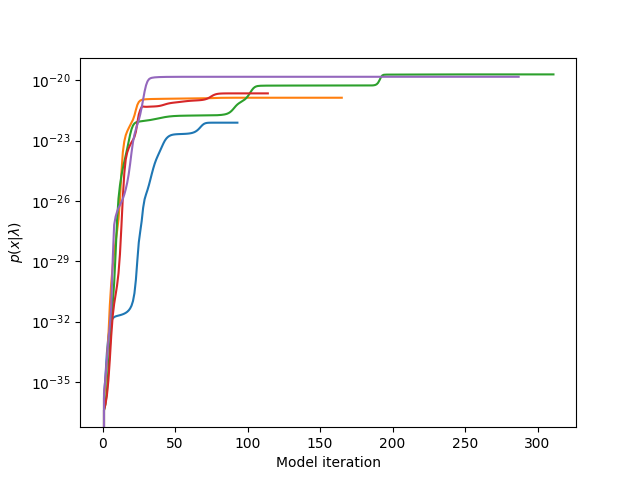
\includegraphics[width=.95\textwidth]{EM2.png}
    \caption{}
    \label{fig:em1}
    \end{center}
    \end{subfigure}%
    \begin{subfigure}{.5\textwidth}
        \begin{center}
        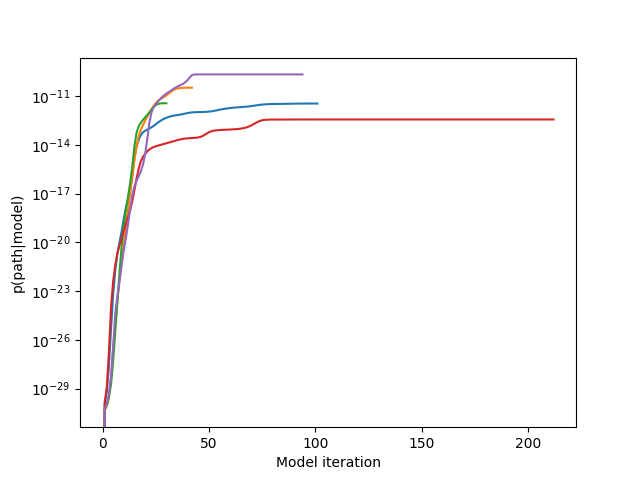
\includegraphics[width=.95\textwidth]{EM.png}
        \caption{}
        \label{fig:em2}
    \end{center}
        \end{subfigure}%
        \caption{Convergence of $p(x|\lambda)$ to local maxima for 2 values of $x$ each using 5 randomly initialised $\lambda$.}
    \label{fig:em}
    \end{center}
    \end{figure}